% Auto-generated by experiments/build_disentanglement_figure.py
\begin{figure}[!htb]
\centering
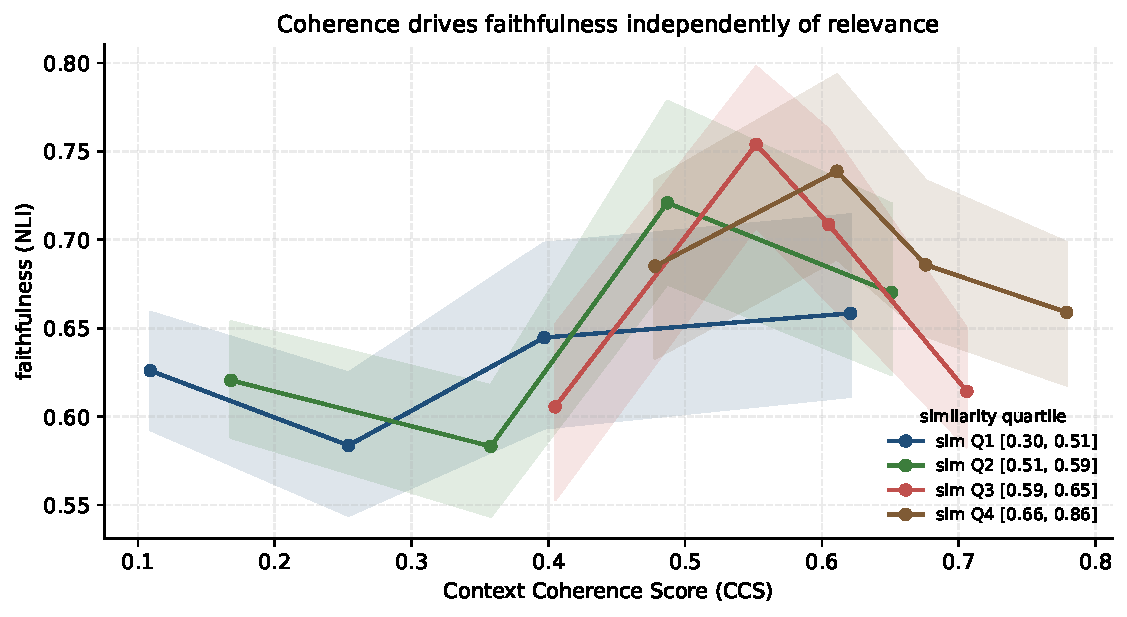
\includegraphics[width=0.96\linewidth]{figures/disentanglement.pdf}
\caption{\textbf{Coherence is causally distinct from relevance.} Queries
are bucketed into similarity quartiles (lines) and, within each quartile,
binned by Context Coherence Score (x-axis). Faithfulness varies
meaningfully along the coherence axis \emph{even at fixed similarity
quartiles}: at high CCS the curves rise toward $0.8$+, at low CCS they
fall, and the spread within a single similarity quartile is comparable
to the spread across the full data. If coherence were a re-statement of
relevance, the lines would be flat. Shaded bands are 95\% bootstrap
CIs over $n \geq 3$ queries per cell.}
\label{fig:disentanglement}
\end{figure}
